\label{sec:neonicotinoids}
This section briefly re-examines community 275, discussed in \S\ref{sec:RESEARCHCLUSTERS}. There was not room for this section to be included in the main body, so is included as an appendix. 

Table \ref{tab:com275} details some of the contents of community 275. Most of the articles in community 275 were published by members of staff who are no longer in the department. The only authors currently in the department are Dr. Kalberer (1 out of 15 articles) and Dr. Vignolini (3 out of 15 articles). These two authors work in very different fields. Dr. Vignolini has worked on plant microsctructures (including pollen) and Dr. Kalberer has worked on atmospheric affects of pollen particles. It could be argued that these two researchers could benefit from discussing each others' work. The program has thus found an unexpected, non-obvious link between these researchers. These unexpected links can be extracted as follows:

The co-occurance of authors is represented in $\mathbf{M}^{Auth. Coinc.}$(figure \ref{fig:commHEATMAP} in \S\ref{chapt:ANALYSIS}). To emphasise where authors often appear together in communities but do not collaborate, a more extreme recommendation matrix could be defined, by setting values in $\mathbf{M}^{Auth. Coinc.}$ to zero if the author pair have ever collaborated. 

Because of the UPGMA clustering, the ordering of the authors in the matrix reflects their similarity (authors are adjacent to similar authors), so that pairs near the diagonal are close. If we select the high values that are distant from the diagonal, these are the more `unexpected' pairings. Setting a minimum distance from diagonal of 10 authors (11 was the population of the largest dendrogram branch identified in \ref{fig:LABELLEDDENDRO} so a distance of 10 ensured author pairs in the same branch were not included), the following heatmap (fig \ref{fig:unexpected_links}) of `unexpected' links is created, $\mathbf{M}^{Unexpected}$.
\begin{figure}[H]
    \centering
    \textbf{Heatmap of non-obvious author links $\mathbf{M}^{Unexpected}$}\par\medskip
    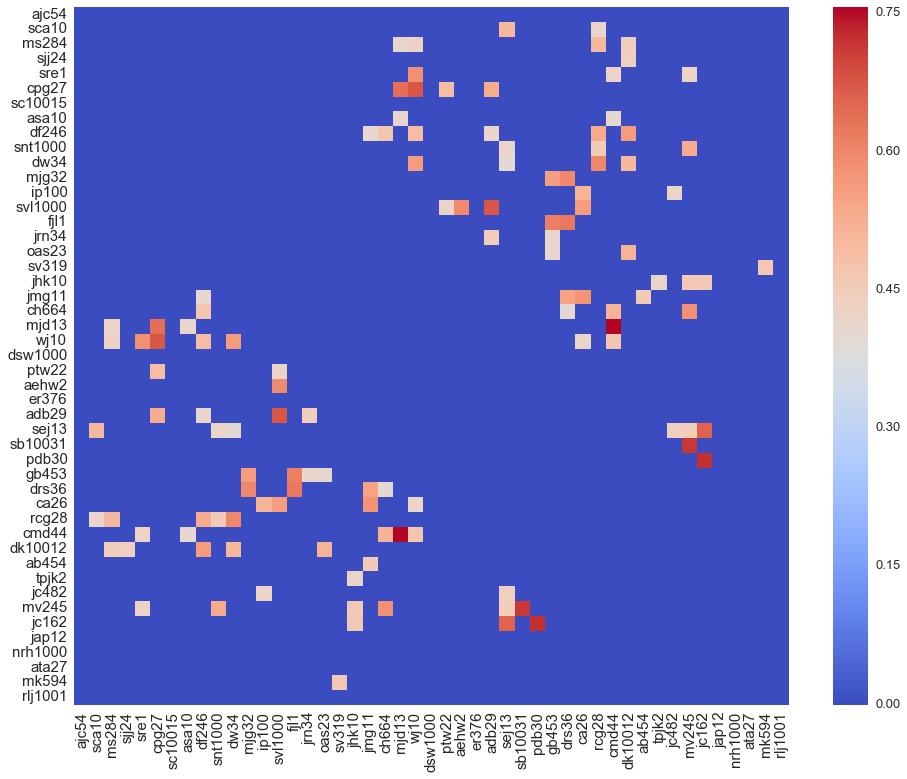
\includegraphics[width=\textwidth]{Appendix/Neonicotinoids/Unexpected_Heatmap.png}
    \caption[Heatmap of Non-Obvious Author Links $\mathbf{M}^{Unexpected}$]{High Values (close to 1, red) indicate that the author pair publish in the same communities but there is no evidence of collaboration (no co-authorship detected). The author pair must also be a distance of 10 authors from the diagonal. Low values indicate low similarity and low evidence of links, or links are `obvious' and therefore not important}
     \label{fig:unexpected_links}
\end{figure}
The top 20 `unexpected' results are shown in table \ref{tab:unexp}. They are ordered by their distance from the diagonal, to attempt to highlight high scores but also the more `unexpected' links.
\begin{table}[H]
\centering
\caption{Top 20 results from $\mathbf{M}^{Unexpected}$}
\label{tab:unexp}
\begin{tabular}{||c|c|c|c||}
\hline
Author 1 & Author 2 & Link Score & Distance from Diagonal\\
\hline
dk10012 & df246 & 0.565 & 28 \\ 
rcg28 & dw34 & 0.598 & 24 \\ 
drs36 & mjg32 & 0.598 & 21 \\ 
mv245 & ch664 & 0.583 & 20 \\
ca26 & svl1000 & 0.561 & 20 \\ 
gb453 & mjg32 & 0.560 & 20 \\ 
drs36 & fjl1 & 0.625 & 18 \\ 
wj10 & sre1 & 0.583 & 18 \\ 
wj10 & cpg27 & 0.674 & 17 \\ 
gb453 & fjl1 & 0.613 & 17 \\ 
mjd13 & cpg27 & 0.641 & 16 \\ 
cmd44 & mjd13 & 0.757 & 14 \\
adb29 & svl1000 & 0.676 & 14 \\ 
ca26 & jmg11 & 0.576 & 14 \\ 
jc162 & sej13 & 0.656 & 13 \\ 
drs36 & jmg11 & 0.550 & 13 \\
aehw2 & svl1000 & 0.596 & 12 \\ 
wj10 & dw34 & 0.564 & 12 \\ 
jc162 & pdb30 & 0.724 & 11 \\ 
mv245 & sb10031 & 0.713 & 11 \\ 
\hline
\end{tabular}
\end{table}
Due to the nature of research in the department, even these `unexpected' pairings can be rationalised. This analysis could be taken further to find the most surprising results using more sophisticated or different techniques. This analysis could be generalised to larger sets of researchers, not just those in the department. The analyses presented in this section and \S\ref{chapt:ANALYSIS} are intended to be useful in their own right, but mainly to serve as the basis for further sophistication.